\chapter{Results}

The aim of this chapter is to explain the procedure followed to evaluate the system throughout the different experiments conducted, concluding with the presentation of the results of each test.

\section{Manual Annotation}

Since the target labels that repressed anger predictor outputs does not match with the classes of either anger and irony binary datasets, a manual annotation of the merged test data must be conducted in order to be able to evaluate the performance of the proposed model. From the 11,074 tweets dedicated for the prediction phase, 1,000 were selected randomly to be part of the manual annotation phase. As the reliability of a single human classification is proven to be low \cite{gonzalez2011identifying} a \acrshort{hit} was conducted to prevent the annotation to be biased.

The \acrshort{hit} was conducted by means of online surveys that were automatically generated as forms by using Google Apps Script. To get a better sense of how difficult the task of repressed anger identification is, the contents of the tweets were presented without anger and irony related hashtags. A total of five non English native collaborators performed the annotation task. The comments received by judges reflect the uncertainty to determine which category a tweet belonged to, as sometimes either context of the tweet was missing or the topic was unknown. We considered valid all the classification which, at least, more that half of the judged agreed. From the 1,000 annotated tweets 824 fulfilled this condition as the remaining 176 was considered ambiguous and thus, discarded from the dataset. The figure \ref{fig:manual_annotation_dataset_distribution} illustrates the distribution of the manually classified dataset that was used to evaluated the performance of the system.

\begin{figure}[!htp]
  \center
  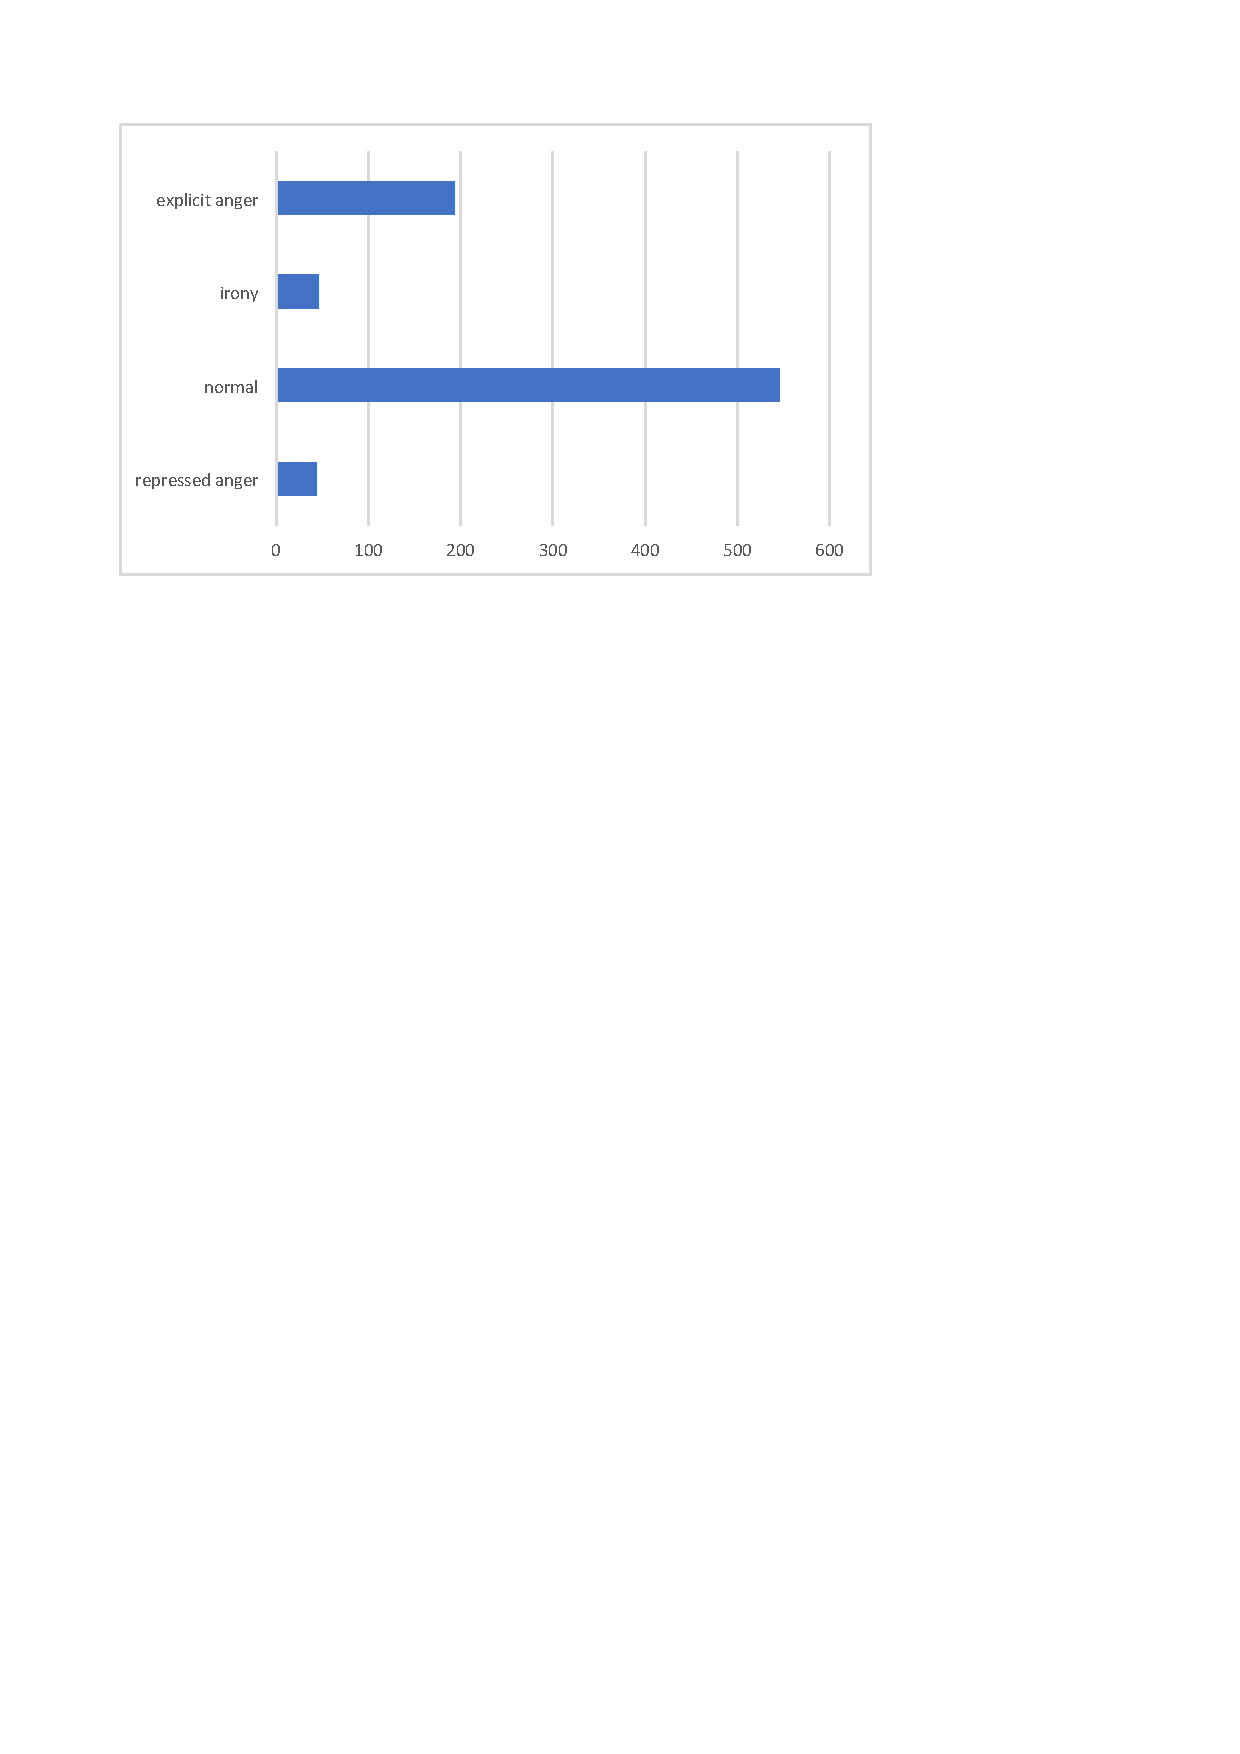
\includegraphics[width=0.6\textwidth]{figures/manual_annotation_dataset_distribution}
  \caption{Manual annotated dataset distribution.}
  \label{fig:manual_annotation_dataset_distribution}
\end{figure}

\section{Experiments}

The project baseline parts from a naive classifier that determines every given instance as the the element with the maximum number of appearances in the dataset, in this case, the \textit{normal} label. From this solution, the designed model is implemented and compared with the baseline to measure how better the proposed solution is. Finally, variations in the proposed procedure are made to try to improve the results.

Because the model designed depends on the word sequence matrices to generate the features maps, from which the model learns, and motivated by the fact that the written style contains features used on oral speech, usually containing spelling mistakes that affect on how the word sequence matrices are generated, the purpose of the modifications done in the procedure aim to improve the data pre-processing and thus, indirectly improve the performance of the model. The experiments conducted in this experiments are the following:

\subsection{Naive classifier}

As explained before, this is the baseline the project bases on to compare the improvement achieved against the proposed solution. It consist of a dummy classifier that assign to each given tweet the \textit{normal} target label.

The results provided make used of the confusion matrix and performance metrics first introduce in the section \ref{general_classificartion_problem_solving}, with all the values rounded to two decimal places.

\begin{table}[!htp]
\centering
  \begin{tabular}{l*4{|>{\centering\arraybackslash}m{\tabwidth}}|}
    \woB{} & \woB{irony} & \woB{normal} & \woB{repressed anger} & \woB{explicit anger} \\ \hhline{~*4{|-}|}
    irony           & 0.0  & \colorme{1.0} & 0.0 & 0.0 \\ \hhline{~*4{|-}|}
    normal          & 0.0  & \colorme{1.0} & 0.0 & 0.0 \\ \hhline{~*4{|-}|}
    repressed anger & 0.0  & \colorme{1.0} & 0.0 & 0.0 \\ \hhline{~*4{|-}|}
    explicit anger  & 0.0  & \colorme{1.0} & 0.0 & 0.0 \\ \hhline{~*4{|-}|}
  \end{tabular}
  \caption{Naive classifier: normalized confusion matrix}
  \label{tab:naive_classifier_confusion_matrix}
\end{table}

\begin{table}[!htp]
\centering
\begin{tabular}{ l|c|c|c|c }
\hline
Class & Average & Precision & Recall & F1-Score  \\ \hline
Irony           & 0.0  & 0.0  & 0.0 & 0.0 \\
Normal          & 1.0  & 0.66 & 1.0 & 0.8 \\
Repressed Anger & 0.0  & 0.0 & 0.0 & 0.0 \\
Explicit anger  & 0.0  & 0.0  & 0.0 & 0.0 \\ \hline
Overall         & 0.66 & 0.16 & 0.25 & 0.2 \\
\hline
\end{tabular}
\caption{Naive classifier: Performance}
\label{tab:naive_performance}
\end{table}

\FloatBarrier

\subsection{Google News word2vec pre-trained model}

This is original proposed solution, first introduced in chapter \ref{proposed_solution}. It uses the publicly available Google News pre-trained model \cite{googleWord2Vec} to generate the word sequence matrices in the pre-processing phase. As with the rest of procedure variations, the performance metrics are divided into two subsection: (i) on the one hand, the evaluation of how the binary classifiers managed to determine independently if a tweet contains anger or irony; (ii) on the other hand, the evaluation of the repressed anger predictor that depends on how well the previous binary classifiers perform to merge their output.

\subsubsection{Binary classifiers}

\begin{table}[!htp]
\centering
  \begin{tabular}{l*2{|>{\centering\arraybackslash}m{\tabwidth}}|}
    \woB{} & \woB{anger} & \woB{no\_anger}        \\ \hhline{~*2{|-}|}
    anger     & \colorme{0.77}  & \colorme{0.23}   \\ \hhline{~*2{|-}|}
    no\_anger & \colorme{0.2}   & \colorme{0.8}    \\ \hhline{~*2{|-}|}
  \end{tabular}
  \caption{Binary anger classifier (Google News): normalized confusion matrix}
  \label{tab:anger_google_confusion_matrix}
\end{table}

\begin{table}[!htp]
\centering
\begin{tabular}{ l|c|c|c|c }
\hline
Class & Average & Precision & Recall & F1-Score  \\ \hline
anger     & 0.77 & 0.79 & 0.77 & 0.78 \\
no\_anger & 0.8  & 0.78 & 0.8  & 0.79 \\ \hline
Overall   & 0.78 & 0.78 & 0.78 & 0.78 \\
\hline
\end{tabular}
\caption{Binary anger classifier (Google News): Performance}
\label{tab:binary_anger_google_news_performance}
\end{table}

\begin{table}[!htp]
\centering
  \begin{tabular}{l*2{|>{\centering\arraybackslash}m{\tabwidth}}|}
    \woB{} & \woB{irony} & \woB{no\_irony}        \\ \hhline{~*2{|-}|}
    irony     & \colorme{0.83}  & \colorme{0.17}   \\ \hhline{~*2{|-}|}
    no\_irony & \colorme{0.14}  & \colorme{0.86}   \\ \hhline{~*2{|-}|}
  \end{tabular}
  \caption{Binary irony classifier (Google News): normalized confusion matrix}
  \label{tab:irony_google_confusion_matrix}
\end{table}

\begin{table}[!htp]
\centering
\begin{tabular}{ l|c|c|c|c }
\hline
Class & Average & Precision & Recall & F1-Score  \\ \hline
irony     & 0.83 & 0.86 & 0.83 & 0.84 \\
no\_irony & 0.86 & 0.83 & 0.86 & 0.84 \\ \hline
Overall   & 0.85 & 0.85 & 0.85 & 0.85 \\
\hline
\end{tabular}
\caption{Binary irony classifier (Google News): Performance}
\label{tab:binary_irony_google_news_performance}
\end{table}

\FloatBarrier

\subsubsection{Repressed anger predictor}

\begin{table}[!htp]
\centering
  \begin{tabular}{l*4{|>{\centering\arraybackslash}m{\tabwidth}}|}
    \woB{} & \woB{irony} & \woB{normal} & \woB{repressed anger} & \woB{explicit anger}    \\ \hhline{~*4{|-}|}
    irony           & \colorme{0.47}  & \colorme{0.3}   & \colorme{0.13}  & \colorme{0.11}  \\ \hhline{~*4{|-}|}
    normal          & \colorme{0.14}  & \colorme{0.56}  & \colorme{0.1}   & \colorme{0.2}   \\ \hhline{~*4{|-}|}
    repressed anger & \colorme{0.23}  & \colorme{0.2}   & \colorme{0.43}  & \colorme{0.14}  \\ \hhline{~*4{|-}|}
    explicit anger  & \colorme{0.09}  & \colorme{0.24}  & \colorme{0.25}  & \colorme{0.42}  \\ \hhline{~*4{|-}|}
  \end{tabular}
  \caption{Google News: normalized confusion matrix}
  \label{tab:google_news_confusion_matrix}
\end{table}

\begin{table}[!htp]
\centering
\begin{tabular}{ l|c|c|c|c }
\hline
Class & Average & Precision & Recall & F1-Score  \\ \hline
Irony           & 0.47 & 0.17 & 0.47 & 0.24 \\
Normal          & 0.56 & 0.82 & 0.56 & 0.67 \\
Repressed Anger & 0.43 & 0.15 & 0.43 & 0.22 \\
Explicit anger  & 0.42 & 0.4  & 0.42 & 0.41 \\ \hline
Overall         & 0.51 & 0.38 & 0.47 & 0.39 \\
\hline
\end{tabular}
\caption{Google News: Performance}
\label{tab:google_news_performance}
\end{table}

\subsection{Fréderic Goding word2vec pre-trained model}

This experiments consist on the same idea as original solution. However, to generate the word sequence matrices, instead of using the Google-News-Vector(300) pre-trained model, which has been created by using the words from the Google News articles, the Fréderic Goding 400 feature pre-trained model \cite{godin2015multimedia} that was generated directly from tweets was used. As tweets are composed by words and a written style that differs from news, using a pre-trained model developed from the content generated from Twitter users could increase the chances of tweet's word appearance in the pre-trained model dictionary and thus, be able to convert more words into a vector space, instead of initialize the unknown words with Zero padding vectors. 

\subsubsection{Binary classifiers}

\begin{table}[!htp]
\centering
  \begin{tabular}{l*2{|>{\centering\arraybackslash}m{\tabwidth}}|}
    \woB{} & \woB{anger} & \woB{no\_anger}        \\ \hhline{~*2{|-}|}
    anger     & \colorme{0.83}  & \colorme{0.17}   \\ \hhline{~*2{|-}|}
    no\_anger & \colorme{0.24}  & \colorme{0.76}   \\ \hhline{~*2{|-}|}
  \end{tabular}
  \caption{Binary anger classifier (Fréderic Goding): normalized confusion matrix}
  \label{tab:anger_frederic_confusion_matrix}
\end{table}

\begin{table}[!htp]
\centering
\begin{tabular}{ l|c|c|c|c }
\hline
Class & Average & Precision & Recall & F1-Score  \\ \hline
anger     & 0.83 & 0.77 & 0.82 & 0.79 \\
no\_anger & 0.76 & 0.82 & 0.76 & 0.79 \\ \hline
Overall   & 0.8  & 0.8  & 0.8  & 0.8  \\
\hline
\end{tabular}
\caption{Binary anger classifier (Fréderic Goding): Performance}
\label{tab:binary_anger_frederic_performance}
\end{table}

\begin{table}[!htp]
\centering
  \begin{tabular}{l*2{|>{\centering\arraybackslash}m{\tabwidth}}|}
    \woB{} & \woB{irony} & \woB{no\_irony}        \\ \hhline{~*2{|-}|}
    irony     & \colorme{0.86}  & \colorme{0.14}   \\ \hhline{~*2{|-}|}
    no\_irony & \colorme{0.14}  & \colorme{0.86}   \\ \hhline{~*2{|-}|}
  \end{tabular}
  \caption{Binary irony classifier (Fréderic Goding): normalized confusion matrix}
  \label{tab:irony_frederic_confusion_matrix}
\end{table}

\begin{table}[!htp]
\centering
\begin{tabular}{ l|c|c|c|c }
\hline
Class & Average & Precision & Recall & F1-Score  \\ \hline
irony     & 0.86 & 0.87 & 0.86 & 0.86 \\
no\_irony & 0.86 & 0.86 & 0.86 & 0.86 \\ \hline
Overall   & 0.86 & 0.86 & 0.86 & 0.86 \\
\hline
\end{tabular}
\caption{Binary irony classifier (Fréderic Goding): Performance}
\label{tab:binary_irony_frederic_performance}
\end{table}

\subsubsection{Repressed anger predictor}

\begin{table}[!htp]
\centering
  \begin{tabular}{l*4{|>{\centering\arraybackslash}m{\tabwidth}}|}
    \woB{} & \woB{irony} & \woB{normal} & \woB{repressed anger} & \woB{explicit anger}    \\ \hhline{~*4{|-}|}
    irony           & \colorme{0.45}  & \colorme{0.3}   & \colorme{0.21}  & \colorme{0.04}  \\ \hhline{~*4{|-}|}
    normal          & \colorme{0.13}  & \colorme{0.65}  & \colorme{0.07}  & \colorme{0.14}  \\ \hhline{~*4{|-}|}
    repressed anger & \colorme{0.34}  & \colorme{0.23}  & \colorme{0.25}  & \colorme{0.18}  \\ \hhline{~*4{|-}|}
    explicit anger  & \colorme{0.1}   & \colorme{0.28}  & \colorme{0.2}   & \colorme{0.41}  \\ \hhline{~*4{|-}|}
  \end{tabular}
  \caption{Fréderic Goding: normalized confusion matrix}
  \label{tab:frederic_goding_confusion_matrix}
\end{table}

\begin{table}[!htp]
\centering
\begin{tabular}{ l|c|c|c|c }
\hline
Class & Average & Precision & Recall & F1-Score  \\ \hline
Irony           & 0.45 & 0.16 & 0.45 & 0.24 \\
Normal          & 0.65 & 0.82 & 0.65 & 0.73 \\
Repressed Anger & 0.25 & 0.11 & 0.25 & 0.15 \\
Explicit anger  & 0.41 & 0.47 & 0.41 & 0.44 \\ \hline
Overall         & 0.56 & 0.39 & 0.44 & 0.39 \\
\hline
\end{tabular}
\caption{Fréderic Goding: Performance}
\label{tab:frederec_performance}
\end{table}

\FloatBarrier

\subsection{Google News word2vec pre-trained model plus spell checker}

This variation consist on adding a spell checker to those words that the Google-New-Vector(300) does not know. The usage of a spell checker would increase the chances of recognizing more words in the pre-trained model's dictionary and thus, initialize its space vector with Word2vec algorithm, helping to obtain new features that would enable the model to achieve better results. As explained in section \ref{sec:solution_prepocessing} of the proposed solution, the spell checker used is based on Peter Norvig's solution. In his blog, he published the code and a language model, big.txt, used to select possible word candidates that correct the grammatical mistakes of the given word. Table \ref{tab:language_model_evaluation} compares the performance obtained by both, big.txt and the self-made language model by executing the evaluation tasks that Norvig designed that checks if the proposed correct word is the expected.

\begin{table}[!htp]
\centering
\begin{tabular}{ l*4{>{\centering\arraybackslash}m{\tabwidth}} }
Model & \woB{No. of words to correct} & \woB{Average of correct words} & \woB{Average of unknown words} & \woB{Words processed per second}  \\ \hline
big.txt language model  & \cuscol{270} & 51\%          & \cuscol{35\%}          & 37 \\
proposed language model & \cuscol{270} & \textbf{75\%} & \cuscol{\textbf{5\%}}  & \textbf{64} \\ \hline
big.txt language model  & \cuscol{400} & 53\%          & \cuscol{32\%}          & 35 \\
proposed language model & \cuscol{400} & \textbf{69\%} & \cuscol{\textbf{7\%}}  & \textbf{63} \\
\hline
\end{tabular}
\caption{Language model evaluation results}
\label{tab:language_model_evaluation}
\end{table}

\clearpage

\subsubsection{Binary classifiers}

\begin{table}[!htp]
\centering
  \begin{tabular}{l*2{|>{\centering\arraybackslash}m{\tabwidth}}|}
    \woB{} & \woB{anger} & \woB{no\_anger}        \\ \hhline{~*2{|-}|}
    anger     & \colorme{0.76}  & \colorme{0.24}   \\ \hhline{~*2{|-}|}
    no\_anger & \colorme{0.19}  & \colorme{0.81}   \\ \hhline{~*2{|-}|}
  \end{tabular}
  \caption{Binary anger classifier (Google News + spell checker): normalized confusion matrix}
  \label{tab:anger_spell_confusion_matrix}
\end{table}

\begin{table}[!htp]
\centering
\begin{tabular}{ l|c|c|c|c }
\hline
Class & Average & Precision & Recall & F1-Score  \\ \hline
anger     & 0.76 & 0.79 & 0.75 & 0.79 \\
no\_anger & 0.81 & 0.77 & 0.81 & 0.79 \\ \hline
Overall   & 0.78 & 0.78 & 0.78 & 0.78 \\
\hline
\end{tabular}
\caption{Binary anger classifier (Google News + spell checker): Performance}
\label{tab:binary_anger_spell_performance}
\end{table}

\begin{table}[!htp]
\centering
  \begin{tabular}{l*2{|>{\centering\arraybackslash}m{\tabwidth}}|}
    \woB{} & \woB{irony} & \woB{no\_irony}        \\ \hhline{~*2{|-}|}
    irony     & \colorme{0.83}  & \colorme{0.17}   \\ \hhline{~*2{|-}|}
    no\_irony & \colorme{0.12}  & \colorme{0.88}   \\ \hhline{~*2{|-}|}
  \end{tabular}
  \caption{Binary irony classifier (Google News + spell checker): normalized confusion matrix}
  \label{tab:irony_spell_confusion_matrix}
\end{table}

\begin{table}[!htp]
\centering
\begin{tabular}{ l|c|c|c|c }
\hline
Class & Average & Precision & Recall & F1-Score  \\ \hline
irony     & 0.83 & 0.87 & 0.82 & 0.84 \\
no\_irony & 0.88 & 0.83 & 0.88 & 0.85 \\ \hline
Overall   & 0.85 & 0.85 & 0.85 & 0.85 \\
\hline
\end{tabular}
\caption{Binary irony classifier (Google News + spell checker): Performance}
\label{tab:binary_irony_spell_performance}
\end{table}

\FloatBarrier

\subsubsection{Repressed anger predictor}

\begin{table}[!htp]
\centering
  \begin{tabular}{l*4{|>{\centering\arraybackslash}m{\tabwidth}}|}
    \woB{} & \woB{irony} & \woB{normal} & \woB{repressed anger} & \woB{explicit anger}    \\ \hhline{~*4{|-}|}
    irony           & \colorme{0.47}  & \colorme{0.3}   & \colorme{0.13}  & \colorme{0.11}  \\ \hhline{~*4{|-}|}
    normal          & \colorme{0.16}  & \colorme{0.59}  & \colorme{0.08}  & \colorme{0.17}  \\ \hhline{~*4{|-}|}
    repressed anger & \colorme{0.3}   & \colorme{0.18}  & \colorme{0.43}  & \colorme{0.09}  \\ \hhline{~*4{|-}|}
    explicit anger  & \colorme{0.08}  & \colorme{0.25}  & \colorme{0.27}  & \colorme{0.4}   \\ \hhline{~*4{|-}|}
  \end{tabular}
  \caption{Google News + spell checker: normalized confusion matrix}
  \label{tab:spell_confusion_matrix}
\end{table}

\begin{table}[!htp]
\centering
\begin{tabular}{ l|c|c|c|c }
\hline
Class & Average & Precision & Recall & F1-Score  \\ \hline
Irony           & 0.47 & 0.16 & 0.47 & 0.24 \\
Normal          & 0.59 & 0.82 & 0.59 & 0.69 \\
Repressed Anger & 0.43 & 0.16 & 0.43 & 0.23 \\
Explicit anger  & 0.4  & 0.43 & 0.4 & 0.42 \\ \hline
Overall         & 0.53 & 0.39 & 0.47 & 0.39 \\
\hline
\end{tabular}
\caption{Google News + spell checker: Performance}
\label{tab:spell_performance}
\end{table}

\FloatBarrier

\section{Result summary}

This section aims to summarize the relevant information from all the scores presented throughout the chapter. Table \ref{tab:represed_anger_performance} illustrates how each model has performed on detecting repressed anger target label, while table \ref{tab:overall_performance} compares the overall performance of each model.

\begin{table}[!htp]
\centering
\begin{tabular}{ l|c|c|c|c }
\hline
Model & Average & Precision & Recall & F1-Score  \\ \hline
Naive classifier    & 0.0           & 0.0           & 0.0  & 0.0 \\
Google News         & \textbf{0.43} & 0.15          & \textbf{0.43} & 0.22 \\
Fréderic Goding     & 0.25          & 0.11          & 0.25          & 0.15 \\
Google News + spell & \textbf{0.43} & \textbf{0.16} & \textbf{0.43} & \textbf{0.23} \\
\hline
\end{tabular}
\caption{Repressed anger performance comparison}
\label{tab:represed_anger_performance}
\end{table}

\begin{table}[!htp]
\centering
\begin{tabular}{ l|c|c|c|c }
\hline
Model & Average & Precision & Recall & F1-Score  \\ \hline
Naive classifier    & \textbf{0.66} & 0.16          & 0.25 & 0.2 \\
Google News         & 0.51          & 0.38          & \textbf{0.47} & \textbf{0.39} \\
Fréderic Goding     & 0.56          & \textbf{0.39} & 0.44          & \textbf{0.39} \\
Google News + spell & 0.53          & \textbf{0.39} & \textbf{0.47} & \textbf{0.39} \\
\hline
\end{tabular}
\caption{Overall model performance comparison}
\label{tab:overall_performance}
\end{table}

\iffalse

Dataset manual classification

Since I generate a new random dataset with no hashtags I had to start the manual classification again.

Manually classified 300 tweets by myself. 

Collaborators have classified 100 tweets (validation).

My goal is to have at least 1000 tweets classified and validated.

Processing the form results (I)

Background: In the forms I asked 2 questions: (I) to classify the sentence and (II) if the sentence was from the irony tweet downloader task I also ask them if the tweet was really ironic instead of talking about irony. This would help me to correct the misclassified tweets in the automatic process.
Difficulties found by the classifiers:  
Some of the tweets are answers to other messages, without that context is difficult to classify current tweet properly.
To check if a tweet is ironic, on some tweets they lack information about the topic to judge properly.
After finished my part of the manual classification, while the collaborators keep sending me more form responses, I started programming the module that processes the results and incorporates them into my CSV for later use in the validation of the system.

[image of generated excel from google form responses]

From the 11,074 tweets dedicated for the prediction phase 1,000 were manually classified. From the obtained responses only those tweets that more than half of the submitters were chosen, the rest (176) were considered ambiguous.
In the end the amount of tweets available for the evaluation process were 824 with the following distribution:
Explicit anger: 193, Irony: 47, Repressed anger: 44 and Normal: 546

[CHECK WHY AMBIGOUOUS NUMBER IS 176 BUT 830 TWEETS ARE IN DATASET INSTEAD 824]

Accuracy: 0.5144578313
Recall(macro): 0.4695591165
Precision(macro): 0.3846361992
F1-Score(macro): 0.3871343406

Trying a new pre-trained word2vec model (I)

Up to know I have been using Google’s publicly available 300 feature, pre-trained word2vec model that has been trained from the english text extracted from Google News.
However, this news tend to be written in a style that differs from how tweet are. Usually tweets contain terms used in spoken English that do not appear in the news. This is the reason why a important amount of theses words are not presented in the Google’s model. Apart from trying to correct the word spelling and use a slang dictionary, using a model that have been trained with actual tweets would increase the chances of improving the amount of words used on the dataset presented in the model.
I found a new model, from Fréderic Goding\cite{godin2015multimedia} that has been trained with 400 millions of tweets and uses 400 features.

Not enough RAM Memory

I encounter a few problems to run the whole process with the new model in two steps: (I) generating binary anger dataset’s word embeddings and (II) compiling the CNN for the first time to train the anger classifier. In both processes the ram of the current GPGPU system is enough to complete these tasks. 
For the word2vec module, before I the GPGPU system was ordered I was working with xe5 server with 128GB of RAM. Therefore, I focus the implementation of the module in execution speed, not on memory consumption. But for the GPGPU system, since the memory is limited I optimize it as much as I could without sacrificing the initial speed design. I managed to make it work with Google word2vec pre-trained module, but for twitter it is not enough.

Memory consumption and xe5 execution time
I run the word2vec over the binary anger dataset on xe5 and check its memory consumption check the amount of memory need to complete that task. The maximum peak was around 43GB of RAM. Since in this process only CPU and RAM are involved the execution time is more or less the same as in the GPGPU system.
For the CNN compilation and training the peak was 30GB of RAM on xe5. Even if the GPGPU does have 31.3GB of memory available, it does still crash. Forums on the internet refer to this error to not having enough RAM or powerful CPU. xe5 expent almost 2 hours to finish the training of the CNN. When the same task with binary irony dataset, that luckily does work under the amount of RAM (\~8,000 tweet less) available usually takes around 6 minutes.

Results comparison
Accuracy: 0.5626506024
Recall(macro): 0.4403748582
Precision(macro): 0.3916296856
F1-Score(macro): 0.390081225

[images of normalized confusion matrix from google and twitter model]

\fi